\documentclass{beamer}
\usepackage{tikz}
\usepackage{lmodern}
\usepackage[absolute,overlay]{textpos}
\usetikzlibrary{shapes,arrows}
\usetikzlibrary{petri}
\usetikzlibrary{automata}

\title{Suppression of Variation in Cell-Size: A Control Theoretic Approach}
\author{Dilawar Singh}

\begin{document}

\begin{frame}

    \maketitle

    Building over a recent work \cite{paulsson}, we explored possibility of
    creating networks of small network which can be used to control cell
    size. We explored few network topologies of a simple control network
    which can keep the size of the cell at a fixed value while giving a
    upper bound on the size of the Endosome. We also wrote a skeleton for
    simulating these topologies in an event-driven simulation environment
    (SystemC library of C++) \cite{github}.

\end{frame}

%% Slide 2.


\begin{frame}{Network under study}
    \begin{figure}
        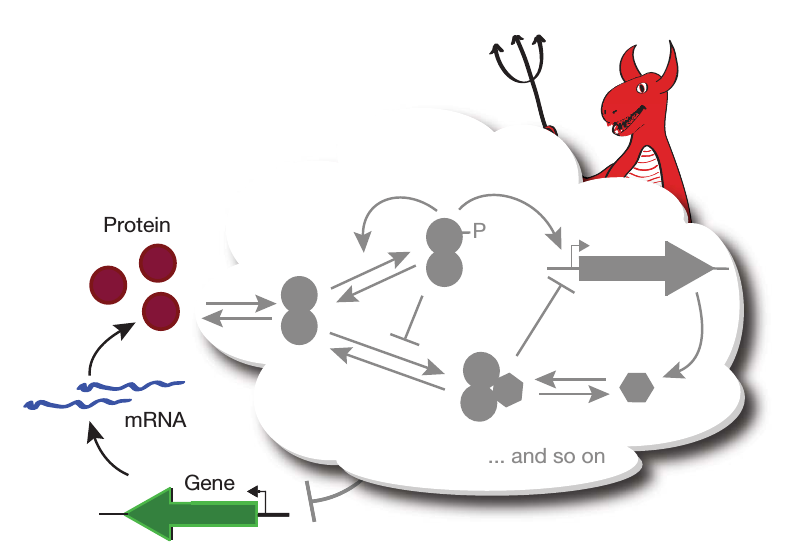
\includegraphics[width=0.5\textwidth]{./fig_mrna_protein.png}
        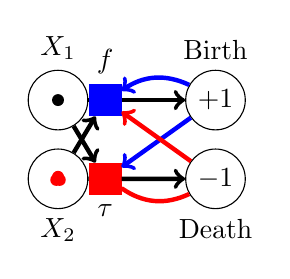
\begin{tikzpicture}[scale=0.2]
            ]
            \node[place,tokens=1,label=above:$X_1$] (X1) at (0,0) {};
            \node[place,colored tokens={red,red,red},label=below:$X_2$] (X2) at (0,-5) {};

            \node[transition,blue,fill,label=above:$f$] (birth) at (3,0) {};
            \node[transition,red,fill,label=below:$\tau$] (death) at (3,-5) {};

            \node[place,label=above:Birth] (Xb) at (10,0) {$+1$};
            \node[place,label=below:Death] (Xd) at (10,-5) {$-1$};


            \draw[ultra thick,->] (X1) to (birth) to (Xb);
            \draw[ultra thick,->] (X1) to  (death);

            \draw[ultra thick,->] (X2) to (death)  to (Xd);
            \draw[ultra thick,->] (X2) to (birth);

            \draw[ultra thick,->,blue] (Xb) to [bend right]  (birth);
            \draw[ultra thick,->,blue] (Xb) to (death);

            \draw[ultra thick,red,->] (Xd) to [bend left] (death) (Xd) to (birth);

        \end{tikzpicture} 


        \caption{\small On left, mRNA/Protein network. In
            our scheme $X_1$ is mRNA and $X_2$ is its protein. Genes are
            intermediate variables which are not shown in network.
            Intermediate variable appears only in feedback path. On right,
        an equivalent Petri net with some details omitted. }
    \label{fig:demon} \end{figure}

    \begin{eqnarray*}
        \tiny
        X_1 \xrightarrow{f'(x_2(-\infty,t))} X_1 + 1 \qquad X_1 \xrightarrow{\tau_{x_1}} X_1 -1 \\
        X_2 \xrightarrow{f(x_1)} X_2 + 1 \qquad X_2 \xrightarrow{\tau_{x_2}} X_2 - 1
    \end{eqnarray*}
\end{frame}

\begin{frame}
    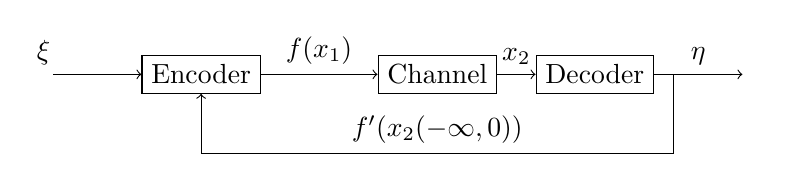
\begin{tikzpicture}[scale=1]
        % This one is information theory approach
        \tikzstyle{block} = [draw,rectangle,];

        \node (input) at (-2,0) {};
        \node (input_midway) at (-1,0) {};
        \node[block] (encoder) at (0,0) {Encoder};
        \node[block,right of=encoder] (channel)  at (2,0) {Channel};
        \node[block,right of=channel,] (decoder) at (4,0)  {Decoder};
        \node[right of=decoder,] at (6,0) (output) {};
        \node[right of=decoder,] (output_mid) {};


        \draw[->] (input) node[above] {$\xi$} -- (encoder);
        \draw[->] (encoder) -- node[above] {$f(x_1)$} (channel);
        \draw[->] (channel) -- node[above] {$x_2$} (decoder);
        \draw[->] (decoder) --  node[above] {$\eta$} (output);

        \draw[->] (output_mid) -| ++(0,-1) -- ++(-3,0) node[above] {$f'(x_2(-\infty,0))$} -| (encoder);

    \end{tikzpicture}

    \def\mean#1{\left< #1 \right>}
    \begin{equation}
        C = \mean{f}\log(1+\frac{\sigma_f^2}{\mean{f}^2})
    \end{equation}

\end{frame}


\begin{frame}
    \frametitle{The bounds}

    The following stochastic equation describes $x_1$.
    \def\mean#1{\left< #1 \right>}
    \begin{equation}
        dx_1 = (\frac{f'-x_1}{\tau _1}) dt + \sqrt{2\mean{x_1}/\tau_1}dw
    \end{equation}

    Following result \cite{paulsson} sets the bound on the variation on
    $x_1$ for the given optimal rate function $f'$ and any $\tau_2$.

    \begin{equation}
        \frac{\sigma_{x_1}^2}{\mean{x_1}} \geq \frac{1}{\sqrt{N_1N_2}}
    \end{equation}

\end{frame}
 

\end{document}
